% Results.

\section{Results}\label{sec:results}

\subsection{Baked cases}\label{sec:results-bake}

Each case is computed offline with every method valid for it (the seed is stated in each manifest), checked against its expected ranges, and committed as a manifest and a trace of at most \liveTraceKiB{} KiB. Table~\ref{tab:calibration} compares the calibration case with the published rows of Di Leonardo et al.~\cite{dileonardo}: the uniformity order of the Gerchberg--Saxton family (plain GS, the adaptive form, weighted GS) and the weighted-GS uniformity are reproduced, as are the lowest uniformity of the superposition and the lowest efficiency of the random mask, while the order of the two random baselines is reversed (random superposition has the higher uniformity here, \calUTwo{} against \calUThree, and the lower in the source, \pubUTwo{} against \pubUThree); the efficiencies of the GS family are lower than published because the engine's Gaussian input beam lowers the efficiency below the flat-beam value by the scale of the single-trap reference level, whereas the source uses a flat beam (the flat-beam test of plain GS gives \accFourFlatEff{} efficiency and \accFourFlatUni{} uniformity; Table~\ref{tab:acceptance}). The uniformity of random superposition and of the random mask differs from the published values on the engine's smaller grid, as the acceptance test of those methods states. The table also gives the phase-fixed weighted GS, which has no published row on this task and leaves a mean spread of \calSigmaSeven{} percent over the three seeds, with a seed range from \calSigmaSevenLo{} to \calSigmaSevenHi{} percent.

\begin{table}[t]\centering\footnotesize
\caption{Calibration case C12 (10 $\times$ 10 traps at eight Fourier units): efficiency $e$ and uniformity $u$ of the analytic and Gerchberg--Saxton baselines, the mean over the three seeds of the canonical bake (the range over the seeds in brackets for $u$ and $\sigma$), against the values published by Di~Leonardo et al.\ for the same task.}\label{tab:calibration}
\begin{tabular}{@{}l r r r r r@{}}\toprule Method & $e$ (baked) & $u$ (baked) & $\sigma$ (\%) & $e$ (published) & $u$ (published)\\\midrule
M01 & 0.328 & 0.000 [0.000, 0.000] & 268.79 [268.79, 268.79] & 0.29 & 0.01\\
M02 & 0.736 & 0.183 [0.148, 0.202] & 40.66 [37.40, 43.84] & 0.69 & 0.01\\
M03 & 0.010 & 0.063 [0.050, 0.077] & 50.97 [47.50, 54.25] & 0.01 & 0.58\\
M04 & 0.817 & 0.575 [0.506, 0.640] & 18.49 [16.37, 19.97] & 0.94 & 0.60\\
M05 & 0.813 & 0.696 [0.637, 0.738] & 12.60 [11.81, 13.76] & 0.93 & 0.79\\
M06 & 0.801 & 0.972 [0.970, 0.975] & 1.15 [1.02, 1.41] & 0.93 & 0.99\\
M07 & 0.792 & 0.990 [0.970, 1.000] & 0.51 [0.01, 1.48] & n/a & n/a\\
\bottomrule\end{tabular}\end{table}

\begin{table}[t]\centering\scriptsize\setlength{\tabcolsep}{3pt}
\caption{Baked results per case at the case budget, the mean over the three seeds of the canonical bake with the range over the seeds in brackets: the method with the lowest mean relative standard deviation among those with at least half the best mean efficiency, and the phase-fixed weighted GS and plain GS rows where they ran. $e$ efficiency, $\sigma$ relative standard deviation of the trap intensities (\%).}\label{tab:results}
\begin{tabular}{@{}l >{\raggedright\arraybackslash}p{0.14\textwidth} r r r r r@{}}\toprule & & & & \multicolumn{2}{c}{Phase-fixed weighted GS} & \\
\cmidrule(lr){5-6} Case & Best & $e$ & $\sigma$ & $\sigma$ & $e$ & GS $\sigma$\\\midrule
C01 & direct search & 0.650 & $<$0.01 [$<$0.01, $<$0.01] & $<$0.01 [$<$0.01, 0.01] & 0.788 & 17.20 [7.34, 23.68]\\
C02 & direct search & 0.649 & 0.01 [0.01, 0.01] & 0.38 [0.01, 0.85] & 0.792 & 17.28 [15.99, 19.48]\\
C03 & phase-fixed weighted GS & 0.794 & 0.42 [0.20, 0.66] & 0.42 [0.20, 0.66] & 0.794 & 17.81 [17.08, 18.68]\\
C04 & shaped potential & n/a & n/a & n/a & n/a & n/a\\
C05 & direct search & 0.679 & 0.01 [0.01, 0.01] & n/a & n/a & 19.35 [16.75, 22.37]\\
C06 & phase-fixed weighted GS & 0.701 & $<$0.01 [$<$0.01, $<$0.01] & $<$0.01 [$<$0.01, $<$0.01] & 0.701 & 8.23 [7.33, 9.29]\\
C07 & direct search & 0.638 & $<$0.01 [$<$0.01, $<$0.01] & $<$0.01 [$<$0.01, 0.01] & 0.785 & 18.19 [13.36, 22.48]\\
C08 & device-aware weighted GS & 0.655 & 6.50 [5.91, 7.04] & 13.21 [13.05, 13.42] & 0.678 & 24.27 [21.62, 28.01]\\
C09 & Zernike correction & 0.799 & 0.33 [0.08, 0.68] & 6.16 [4.66, 7.09] & 0.447 & 15.35 [14.98, 15.71]\\
C10 & flicker-bounded phase-continuous sequence & 0.793 & 0.02 [$<$0.01, 0.06] & 0.02 [0.01, 0.04] & 0.792 & n/a\\
C12 & phase-fixed weighted GS & 0.792 & 0.51 [0.01, 1.48] & 0.51 [0.01, 1.48] & 0.792 & 18.49 [16.37, 19.97]\\
C13 & phase-fixed weighted GS & 0.725 & 0.26 [0.18, 0.30] & 0.26 [0.18, 0.30] & 0.725 & 10.97 [10.62, 11.17]\\
C14 & weighted GS & 0.785 & 0.49 [0.32, 0.59] & n/a & n/a & 16.91 [15.26, 18.41]\\
\bottomrule\end{tabular}\end{table}


Table~\ref{tab:results} summarizes the baked cases. Where both ran (\hlN{} cases of the bake, among them the device-limited case C08 and the aberrated case C09), phase-fixed weighted GS leaves a median relative standard deviation of \hlSigmaMseven{} percent against \hlSigmaMfour{} percent for plain GS, each the median over the cases of the mean over the three seeds of the bake; the medians of the single seeds range from \hlSigmaMsevenLo{} to \hlSigmaMsevenHi{} percent and from \hlSigmaMfourLo{} to \hlSigmaMfourHi{} percent, so that the first seed of the bake, the one the manifests hold, gives a lower value for the phase-fixed form (\medSigmaMseven{} percent) than the mean of the three. The mean efficiency of the phase-fixed form lies between \hlEffLo{} (the aberrated case) and \hlEffHi{}. The full matrix of the bake is Table~\ref{tab:bake-sigma} for the spread and Table~\ref{tab:bake-eff} for the efficiency, each cell the mean over the three seeds of the canonical bake with its range. Over the \nTrapCases{} point-trap cases, the weighted GS has a lower mean spread than GS in \winsSixOverFour{} of the \nBothFourSix{} cases where both ran; over the \cmN{} cases where plain GS, weighted GS and the phase-fixed form all ran (one common set, so that the medians are comparable), the median over the cases of the mean spread is \cmSigmaFour{} percent for GS (efficiency \cmEffFour), \cmSigmaSix{} percent for weighted GS (\cmEffSix) and \cmSigmaSeven{} percent for the phase-fixed form (\cmEffSeven), so that the integral feedback of the weights removes more than an order of magnitude of the spread and the freeze of the phase a further factor of a few, at an efficiency that stays within a few hundredths. The analytic baselines show the reverse: the superposition and the random superposition leave the largest spreads, the random mask trades its efficiency (about the inverse of the trap count, Table~\ref{tab:bake-eff}) for a moderate spread that depends on the pixels per trap, and the gradient method conjugate-gradient minimization at the 30-iteration budget of the bake is far from converged, as its method section states. Direct search reaches the smallest spreads on the ideal-device lattices it runs on, at a lower efficiency than the weighted forms, while the knee of the proposed front reaches a spread of the order of the phase-fixed form at the efficiency of the weighted form; the flicker-bounded sequence is scored on its final hologram on the rearrangement case only.

\begin{table}[t]\centering\scriptsize\setlength{\tabcolsep}{3pt}
\caption{Relative standard deviation of the trap intensities (percent), mean over the three seeds of the canonical bake, every method on every point-trap case it ran on; blank cells are methods the case does not run. The seed range of selected cells is in Table~\ref{tab:seeds}.}\label{tab:bake-sigma}
\begin{tabular}{@{}l rrrrrrrrrrrr@{}}\toprule Id & C01 & C02 & C03 & C05 & C06 & C07 & C08 & C09 & C10 & C12 & C13 & C14\\\midrule
M01 & 64 & 274 & 925 & 79 & 27 & 116 &  & 78 &  & 269 & 25 & 69\\
M02 & 35 & 40 & 39 & 43 & 9.5 & 38 &  &  &  & 41 & 14 & 26\\
M03 & 4.4 & 54 &  &  &  & 15 &  &  &  & 51 &  & \\
M04 & 17 & 17 & 18 & 19 & 8.2 & 18 & 24 & 15 &  & 18 & 11 & 17\\
M05 & 8.6 & 13 &  &  &  & 14 &  &  &  & 13 &  & \\
M06 & 0.009 & 1.2 & 1.1 & 1.2 & 0.13 & 0.76 & 14 & 6 & 0.98 & 1.1 & 0.66 & 0.49\\
M07 & 0.0035 & 0.38 & 0.42 &  & $<$0.001 & 0.004 & 13 & 6.2 & 0.022 & 0.51 & 0.26 & \\
M09 & $<$0.001 & 0.014 &  & 0.0064 & 0.0024 & 0.0029 &  &  &  &  &  & \\
M10 & 52 & 41 &  & 53 & 45 & 63 & 32 &  &  &  &  & 30\\
M11 & 1.3 & 2.5 &  & 1.8 &  & 2.5 &  &  &  &  &  & 2\\
M12 & 18 & 20 & 20 &  &  &  &  &  &  &  & 19 & \\
M13 &  &  &  &  &  &  & 25 &  &  &  &  & \\
M14 &  &  &  &  &  &  &  & 0.33 &  &  &  & \\
M15 &  &  &  & 1.2 & 0.13 &  &  &  &  &  &  & \\
M17 &  &  &  &  &  &  &  &  &  &  &  & 36\\
M19 &  &  &  & 62 &  &  &  &  &  &  &  & 16\\
B1 &  &  &  &  &  &  & 6.5 &  &  &  &  & \\
B2 &  &  &  &  &  &  &  &  & 0.02 &  &  & \\
B3 & 0.0033 & 0.38 & 0.42 &  &  & 0.004 &  &  &  &  & 0.26 & \\
B4 & 0.59 & 0.85 &  &  &  & 0.98 & 13 & 5.3 &  &  &  & \\
B5 & 0.031 & 0.53 &  & 0.66 &  & 0.54 &  &  &  &  &  & \\
\bottomrule\end{tabular}\end{table}

\begin{table}[t]\centering\scriptsize\setlength{\tabcolsep}{3pt}
\caption{Efficiency of the same runs as Table~\ref{tab:bake-sigma}: mean over the three seeds of the canonical bake, the fraction of the input power in the traps, scored on the case's own device.}\label{tab:bake-eff}
\begin{tabular}{@{}l rrrrrrrrrrrr@{}}\toprule Id & C01 & C02 & C03 & C05 & C06 & C07 & C08 & C09 & C10 & C12 & C13 & C14\\\midrule
M01 & 0.45 & 0.28 & 0.19 & 0.45 & 0.59 & 0.35 &  & 0.21 &  & 0.33 & 0.60 & 0.50\\
M02 & 0.72 & 0.74 & 0.74 & 0.77 & 0.69 & 0.73 &  &  &  & 0.74 & 0.69 & 0.70\\
M03 & 0.09 & 0.01 &  &  &  & 0.04 &  &  &  & 0.01 &  & \\
M04 & 0.80 & 0.82 & 0.82 & 0.91 & 0.71 & 0.81 & 0.70 & 0.46 &  & 0.82 & 0.74 & 0.80\\
M05 & 0.81 & 0.81 &  &  &  & 0.80 &  &  &  & 0.81 &  & \\
M06 & 0.80 & 0.80 & 0.81 & 0.89 & 0.70 & 0.80 & 0.69 & 0.45 & 0.80 & 0.80 & 0.74 & 0.79\\
M07 & 0.79 & 0.79 & 0.79 &  & 0.70 & 0.79 & 0.68 & 0.45 & 0.79 & 0.79 & 0.72 & \\
M09 & 0.65 & 0.65 &  & 0.68 & 0.64 & 0.64 &  &  &  &  &  & \\
M10 & 0.17 & 0.26 &  & 0.21 & 0.16 & 0.19 & 0.31 &  &  &  &  & 0.31\\
M11 & 0.79 & 0.76 &  & 0.82 &  & 0.77 &  &  &  &  &  & 0.75\\
M12 & 0.81 & 0.81 & 0.81 &  &  &  &  &  &  &  & 0.74 & \\
M13 &  &  &  &  &  &  & 0.42 &  &  &  &  & \\
M14 &  &  &  &  &  &  &  & 0.80 &  &  &  & \\
M15 &  &  &  & 0.89 & 0.70 &  &  &  &  &  &  & \\
M17 &  &  &  &  &  &  &  &  &  &  &  & 0.40\\
M19 &  &  &  & 0.53 &  &  &  &  &  &  &  & 0.75\\
B1 &  &  &  &  &  &  & 0.65 &  &  &  &  & \\
B2 &  &  &  &  &  &  &  &  & 0.79 &  &  & \\
B3 & 0.79 & 0.79 & 0.79 &  &  & 0.79 &  &  &  &  & 0.72 & \\
B4 & 0.78 & 0.78 &  &  &  & 0.77 & 0.67 & 0.44 &  &  &  & \\
B5 & 0.80 & 0.80 &  & 0.89 &  & 0.80 &  &  &  &  &  & \\
\bottomrule\end{tabular}\end{table}


The seed-to-seed uncertainty of the bake is read in Table~\ref{tab:seeds}. On the ideal-device grid C02 the weighted methods differ from seed to seed in a spread that is already near or below one percent (the range of the phase-fixed form spans more than an order of magnitude), so a one-seed ranking among them would be fragile; on the device-limited case C08 the ranges are narrow and the methods fall into groups: weighted GS, phase-fixed weighted GS and the aberration-robust hologram keep a spread of the order of ten percent, and the device-aware the device-aware weighted GS lowers it. On C08 phase-fixed weighted GS (phase-fixed weighted GS), which ignores the device, keeps a spread of \bakeCeightMsevenSigma{} percent, and the device-aware weighted GS (the device-aware weighted GS) lowers it to \bakeCeightBOneSigma{} percent, a factor of \bakeCeightRatio{} on the bake's own seed (\bakeCeightRatioThree{} on the ratio of the means of its \bakeCeightSeedsN{} seeds), on that small grid (the larger task of the acceptance gate gives a larger factor; both are reported in the companion manuscript~\cite{companion}). On the aberrated case C09, correction of the Zernike modes (the Zernike correction) restores efficiency and uniformity that the uncorrected methods lose; the proposed aberration-robust hologram scores a lower mean spread than the nominal method on one realization per seed, a smaller factor than its ensemble criterion.

\begin{table}[t]\centering\footnotesize
\caption{Relative standard deviation (percent) of selected methods on three cases: mean over the three seeds of the bake and the minimum and maximum over the seeds in brackets, the uncertainty the bake supports; C02 is the ideal-device grid, C08 the device-limited array, C09 the aberrated array.}\label{tab:seeds}
\begin{tabular}{@{}l rrr@{}}\toprule Id & C02 & C08 & C09\\\midrule
M04 & 17 [16, 19] & 24 [22, 28] & 15 [15, 16]\\
M06 & 1.2 [0.86, 1.5] & 14 [12, 14] & 6 [4.8, 7.3]\\
M07 & 0.38 [0.014, 0.85] & 13 [13, 13] & 6.2 [4.7, 7.1]\\
M11 & 2.5 [2.4, 2.6] &  & \\
B1 &  & 6.5 [5.9, 7] & \\
B4 & 0.85 [0.83, 0.87] & 13 [13, 14] & 5.3 [4.6, 5.8]\\
B5 & 0.53 [$<$0.001, 1.1] &  & \\
\bottomrule\end{tabular}\end{table}


\begin{figure}[t]
\centering
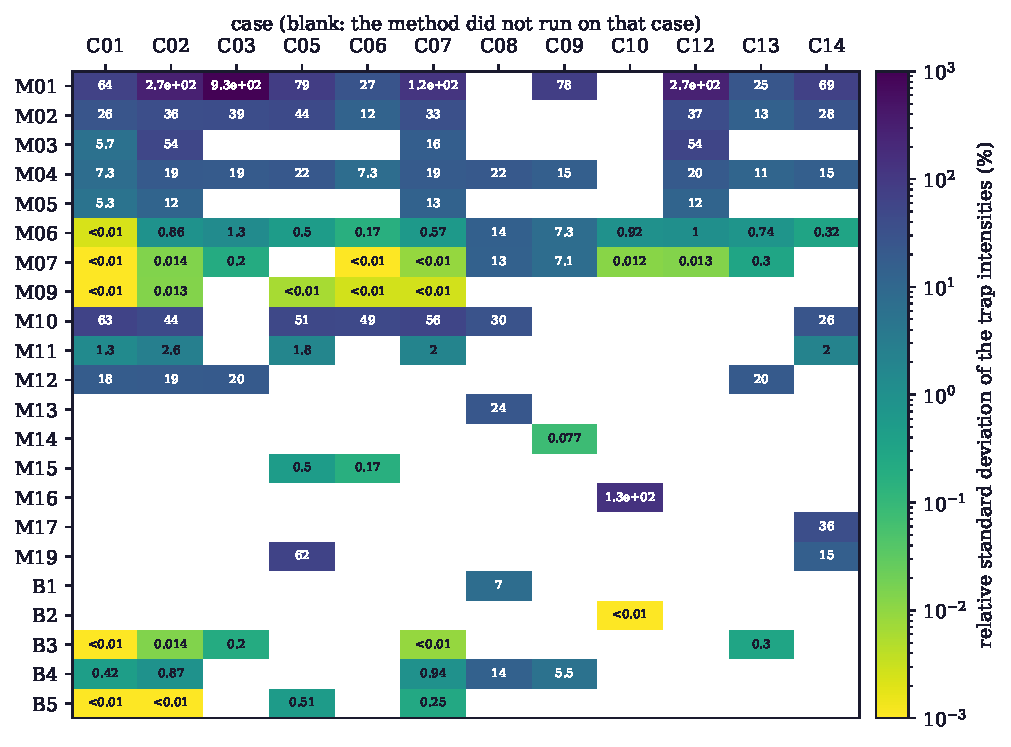
\includegraphics[width=0.92\textwidth]{fig-cases.pdf}
\caption{Relative standard deviation of the trap intensities, every method on every point-trap case of the bake (the shaped-potential case C04 is scored on its signal region and is omitted). Each cell is the mean over the three seeds of the canonical bake of one method at the case budget (the matrix of Table~\ref{tab:bake-sigma}, not the single bake seed of the manifests). Plain Gerchberg--Saxton leaves the largest spreads among the iterative methods; the weighted and phase-fixed forms, the direct search, the Pareto front and the device-aware methods remove most of it where they apply.}
\label{fig:cases}
\end{figure}

Figure~\ref{fig:cases} shows the same matrix of three-seed means as a heat map, which makes the structure visible: the rows of the weighted and optimization methods are dark (low spread) on every ideal-device case where they run, the rows of the analytic baselines are light, and the device-limited and aberrated columns are lighter for every method, which is the cost of the device and of the aberration that the device-aware and robust methods target. Figure~\ref{fig:convergence} follows the spread along the iterations from the baked traces. Each curve is the history that the method reports for itself, which is the quantity the method optimizes. On the ideal-device grid the curves of the weighted and phase-fixed forms fall by orders of magnitude over the budget, GS plateaus at a spread of the order of ten percent, the adaptive form plateaus a little lower, and the Wirtinger descent starts at a large spread and falls steadily. On the device-limited case the picture differs by what each method sees. The weighted and phase-fixed forms keep falling, because their history is measured on the ideal model that they optimize, while the scored spread on the device is the value of Table~\ref{tab:bake-sigma}, of the order of ten percent: this is the gap between equalizing the model and equalizing the device that the device-aware method addresses. The device-aware weighted GS reports its history on the device model and settles at a floor set by that model, and the conjugate-gradient methods are still far from converged at the budget of the bake.

\begin{figure}[t]
\centering
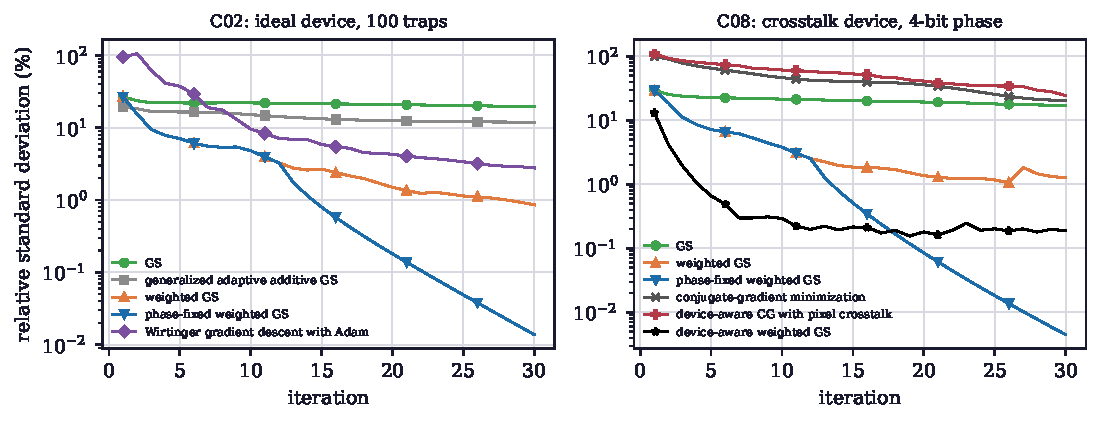
\includegraphics[width=\textwidth]{fig-convergence.pdf}
\caption{Relative standard deviation of the trap intensities against the iteration, read from the baked traces: (a) the ideal-device grid C02 for GS, the adaptive form, weighted GS, phase-fixed weighted GS and Wirtinger descent; (b) the device-limited array C08 for the same family, the conjugate gradient, its device-aware form and the device-aware weighted GS. Each curve is the history the method reports for itself: the ideal model for GS, the adaptive form, weighted GS, phase-fixed weighted GS and the conjugate gradient, the device model for the device-aware conjugate gradient and the device-aware weighted GS. The vertical axis is logarithmic.}
\label{fig:convergence}
\end{figure}

\begin{figure}[t]
\centering
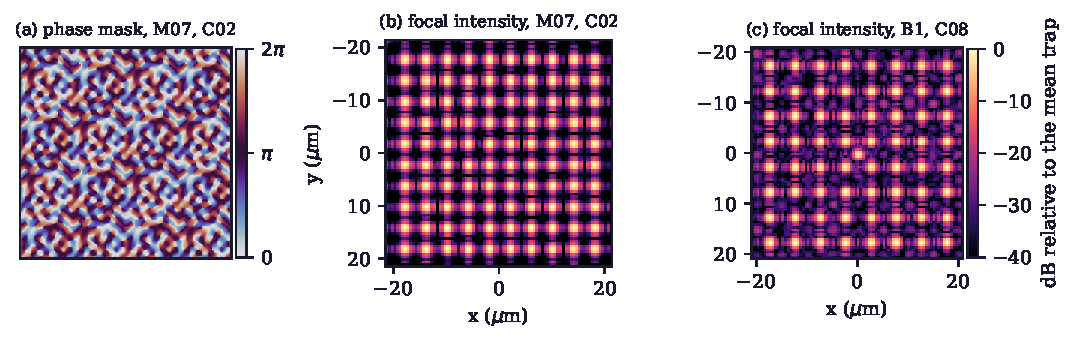
\includegraphics[width=\textwidth]{fig-maps.pdf}
\caption{(a) Phase mask of the reference method on C02. (b) Its focal intensity, in dB relative to the mean trap, on the ideal device: a regular lattice. (c) The focal intensity of the device-aware weighted GS on C08, scored on the device with 4-bit phase, crosstalk and a fill factor of \devcFill: the traps are visible and not equal.}
\label{fig:maps}
\end{figure}

Figure~\ref{fig:maps} shows what the numbers describe in the focal plane: the hologram of the reference method on C02 is a quantized phase mask whose focal intensity is a regular lattice with a faint structure between the traps, and the device-aware hologram on the device-limited case forms traps that are visible but not equal, because the quantizer and the flicker are not modelled by the optimizer. The figure shows one hologram per panel and does not show how the maps change with the method, because the trace carries the maps of the reference method only.

The power budget of the point-trap cases (Table~\ref{tab:power}) separates the light that reaches the traps, the zero order and the ghost traps. On the lattices of cases C02, C03, C07, C08, C12 and C13 the ghost traps hold about an eighth to a fifth of the input power (0.12 to 0.22) for both plain GS and the phase-fixed form, and on the ring-and-line case C06 and the aberrated case C09 they hold 0.42 to 0.46; the zero order is nil except on the nine-trap case C01 (0.09 to 0.11) and on the cases with a high numerical aperture and a device (0.03 and 0.01). The phase-fixed form, which equalizes the traps, sends 0.002 to 0.023 more of the power to ghost traps than plain GS on every case, so that its higher uniformity is paid for by a small loss of efficiency and not by a redistribution to the zero order. The table is read at the bake seed of each case, one seed, and is a description and not an estimate with an interval.

\begin{table}[t]\centering\footnotesize
\caption{Power budget of the point-trap cases at the bake seed (one seed per case): the fraction of the input power in the traps $e$, in the zero order $z_0$ and in the ghost traps $g$ (everything else on the grid, including folded replicas), for plain GS and phase-fixed weighted GS where they ran. The remainder of the power is zero for the plain Fourier form.}\label{tab:power}
\begin{tabular}{@{}l r r r r r r@{}}\toprule & \multicolumn{3}{c}{GS} & \multicolumn{3}{c}{Phase-fixed weighted GS}\\
\cmidrule(lr){2-4}\cmidrule(l){5-7} Case & $e$ & $z_0$ & $g$ & $e$ & $z_0$ & $g$\\\midrule
C01 & 0.819 & 0.108 & 0.120 & 0.817 & 0.091 & 0.122\\
C02 & 0.818 & 0.000 & 0.117 & 0.798 & 0.000 & 0.140\\
C03 & 0.817 & 0.000 & 0.115 & 0.794 & 0.000 & 0.138\\
C06 & 0.710 & 0.000 & 0.449 & 0.704 & 0.000 & 0.461\\
C07 & 0.807 & 0.034 & 0.126 & 0.791 & 0.032 & 0.144\\
C08 & 0.692 & 0.008 & 0.133 & 0.675 & 0.008 & 0.148\\
C09 & 0.458 & 0.000 & 0.423 & 0.453 & 0.000 & 0.430\\
C12 & 0.817 & 0.000 & 0.123 & 0.797 & 0.000 & 0.145\\
C13 & 0.740 & 0.000 & 0.202 & 0.723 & 0.000 & 0.217\\
\bottomrule\end{tabular}\end{table}


\subsection{Feedback and particles}\label{sec:results-feedback}

The emulated camera loop reduces the spread as in the published curves. In the baked traces the relative standard deviation falls from \fbCOneStart{} to \fbCOneEnd{} percent in \fbCOneSteps{} steps on C01, from \fbCTwoStart{} to \fbCTwoEnd{} percent in \fbCTwoSteps{} steps on the $10\times10$ grid C02, from \fbCThreeStart{} to \fbCThreeEnd{} percent in \fbCThreeSteps{} steps on the large array C03, and from \fbCThirteenStart{} to \fbCThirteenEnd{} percent in \fbCThirteenSteps{} steps on the disordered array C13 (Figure~\ref{fig:feedback}). The published closed-loop result of Nogrette et al.~\cite{nogrette} is a trap-depth spread of 19 percent rms reduced to 1.4 percent in 20 iterations; the unit test of the closed-loop method reproduces it within the factor set in the design document (Table~\ref{tab:acceptance}). The loop of the cases differs from the closed-loop method itself: it applies the same factor to the case's weight-aware method and reports the measured spread of the camera readings, which is why the curves of Figure~\ref{fig:feedback} reach a fraction of a percent while the true intensities keep the size of the camera's own gain error. The figure shows the measured spread and not the true one, so it shows that the loop equalizes what the camera sees, which is the property of the published procedure.

\begin{figure}[t]
\centering
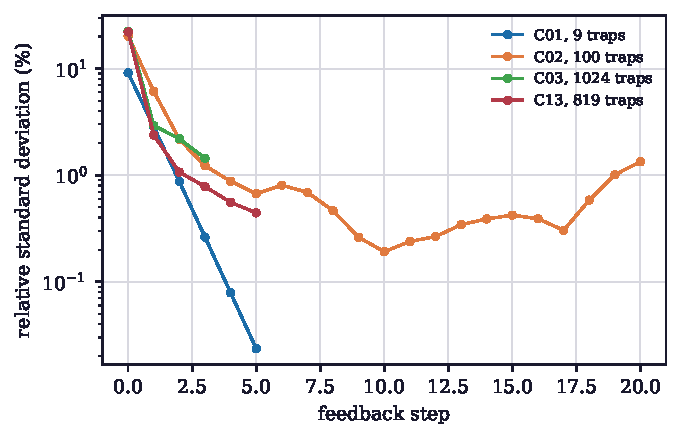
\includegraphics[width=0.62\textwidth]{fig-feedback.pdf}
\caption{Emulated camera feedback: relative standard deviation of the trap intensities against the feedback step, on four cases (baked traces). The measured spread is that of the camera readings divided by the target weights, the quantity the experimenter sees.}
\label{fig:feedback}
\end{figure}

The particle simulations act on the computed traps: C01 carries a bead in the central trap (stiffness \beadKappa{} pN/$\mu$m and a corner frequency of \beadFc{} Hz in the trace) and C03 an atom (a corner frequency of \atomFc{} Hz and a radial trap frequency of \atomOmega{} Hz in the trace); the trap depth follows the intensity~\cite{grimm}, and the bead's spectrum is a Lorentzian whose corner frequency is the stiffness over $2\pi\gamma$~\cite{tolic}, which the particle oracle checks. The fit of a Lorentzian to an average of $n$ power spectra carries a bias of relative size between $-2/n$ and $+1/n$~\cite{norrelykke}; the bounds on the fitted corner frequency, twelve percent in the oracle test and ten percent in the engine's dynamics test, are DinHot's own tolerances for the segment counts those runs use.

\subsection{The benchmark}\label{sec:results-bench}

The protocol of Section~\ref{sec:protocol-bench} gives the benchmark. Table~\ref{tab:benchmark} names, per geometry and device, the published method and the proposed method with the lowest median spread at 100 iterations among those that reach at least half of the cell's best efficiency, and the best method at a time budget of 1~s; Table~\ref{tab:benchmethods} gives the medians of every method over the \benchNPoint{} point-trap geometries, and Figure~\ref{fig:bench} every cell. On the ideal device the best method of a geometry is a published method on \benchWinsIdealPublished{} and a proposed method on \benchWinsIdealProposed{} of the \benchGeoIdeal{} geometries, and on \benchTiesIdeal{} the best published and proposed methods tie below the resolution of the file (0.001 percent); on the C08 device the counts are \benchWinsDevicePublished{} and \benchWinsDeviceProposed{} of \benchGeoDevice{} (the multi-plane geometry has no device rows), with \benchTiesDevice{} ties. The flicker-bounded sequence enters these cells as its static frame, a phase-locked weighted GS, and not as a sequence, which is the quantity of its claim (Section~\ref{sec:b2}). Over the point-trap geometries the lowest median spread on the ideal device is that of \benchBestIdeal{} (\benchBestIdealSigma{} percent at a median efficiency of \benchBestIdealEff{}), and on the C08 device that of \benchBestDevice{} (\benchBestDeviceSigma{} percent at \benchBestDeviceEff{}). The medians of the \benchSpreadIdealN{} methods that keep at least half of the best efficiency span \benchSpreadIdealLow{} to \benchSpreadIdealHigh{} percent on the ideal device and \benchSpreadDeviceLow{} to \benchSpreadDeviceHigh{} percent (\benchSpreadDeviceN{} methods) on the C08 device, where every method runs with its default parameters and only the device-aware ones model the device. The times are wall-clock seconds of the machine that ran the benchmark, under shared load.

\begin{table}[t]\centering\footnotesize
\caption{Benchmark, per geometry and device: the published method and the proposed method with the lowest median relative standard deviation $\sigma$ (\%) at 100 iterations among those that reach at least half of the best median efficiency of the cell, and the best method of all at a time budget of 1~s. Default parameters, medians over the seeds of each cell.}\label{tab:benchmark}
\begin{tabular}{@{}>{\raggedright\arraybackslash}p{0.2\textwidth} l >{\raggedright\arraybackslash}p{0.17\textwidth} >{\raggedright\arraybackslash}p{0.2\textwidth} >{\raggedright\arraybackslash}p{0.2\textwidth}@{}}\toprule Geometry & Device & Published & Proposed & Best at 1 s\\\midrule
G1 Square 10 x 10 & ideal & direct search 0.071 & device-aware weighted GS $<$0.001 & device-aware weighted GS $<$0.001\\
G1 Square 10 x 10 & C08 & Wirtinger gradient descent with Adam 12 & aberration-robust hologram 24 & Wirtinger gradient descent with Adam 20\\
G2 Ring of 36 traps & ideal & phase-fixed weighted GS $<$0.001 & device-aware weighted GS $<$0.001 & device-aware weighted GS $<$0.001\\
G2 Ring of 36 traps & C08 & superposition of prisms and lenses 6.6 & device-aware weighted GS 7.5 & superposition of prisms and lenses 6.6\\
G3 Random 100 traps & ideal & phase-fixed weighted GS $<$0.001 & device-aware weighted GS $<$0.001 & device-aware weighted GS $<$0.001\\
G3 Random 100 traps & C08 & Wirtinger gradient descent with Adam 14 & device-aware weighted GS 4.4 & Wirtinger gradient descent with Adam 20\\
G4 Quasi-periodic 119 & ideal & phase-fixed weighted GS 0.012 & device-aware weighted GS $<$0.001 & device-aware weighted GS $<$0.001\\
G4 Quasi-periodic 119 & C08 & Wirtinger gradient descent with Adam 21 & device-aware weighted GS 81 & conjugate-gradient minimization 76\\
G5 3D lattice 5 x 5 x 3 & ideal & direct search 0.042 & flicker-bounded phase-continuous sequence $<$0.001 & flicker-bounded phase-continuous sequence $<$0.001\\
G6 Large: 32 x 32 and disordered 819 & ideal & direct search 0.15 & device-aware weighted GS $<$0.001 & phase-fixed weighted GS 0.78\\
G6 Large: 32 x 32 and disordered 819 & C08 & Wirtinger gradient descent with Adam 18 & device-aware weighted GS 17 & weighted GS 19\\
G7 Shaped fields (ring, disc, line, LG ring) & ideal & GS 35 & n/a & GS 36\\
G7 Shaped fields (ring, disc, line, LG ring) & C08 & GS 40 & n/a & optimal-transport initialized MRAF 39\\
\bottomrule\end{tabular}\end{table}

\begin{table}[t]\centering\footnotesize
\caption{Benchmark, per method: medians over the point-trap geometries the method ran on (of 6) at 100 iterations with the default parameters, on the ideal device and on the C08 device. $\sigma$ relative standard deviation (\%): the median over the geometries of the cell medians and, in brackets, the median over the geometries of the first and third quartiles over the seeds of each cell; $e$ efficiency; time wall-clock seconds under shared load.}\label{tab:benchmethods}
\begin{tabular}{@{}l r r r r r r@{}}\toprule Id & Geometries & $\sigma$ ideal & $e$ ideal & time (s) & $\sigma$ C08 & $e$ C08\\\midrule
\multicolumn{7}{@{}l}{\textit{Published methods}}\\
M01 & 6 & 136 [66, 136] & 0.399 & 0.0044 & 175 [27, 175] & 0.279\\
M02 & 6 & 25 [19, 33] & 0.710 & 0.0053 & 31 [21, 49] & 0.478\\
M03 & 6 & 78 [75, 82] & 0.015 & 0.068 & 89 [85, 94] & 0.013\\
M04 & 6 & 14 [11, 15] & 0.799 & 0.82 & 31 [22, 33] & 0.523\\
M05 & 6 & 9.1 [7.8, 11] & 0.780 & 1.1 & 24 [21, 30] & 0.514\\
M06 & 6 & 0.3 [0.19, 0.35] & 0.775 & 0.72 & 21 [20, 27] & 0.518\\
M07 & 5 & 0.012 [$<$0.001, 0.17] & 0.751 & 0.55 & 26 [20, 28] & 0.503\\
M08 & 0 & n/a & n/a & n/a & n/a & n/a\\
M09 & 6 & 0.059 [0.057, 0.06] & 0.641 & 58 & 20 [20, 23] & 0.431\\
M10 & 6 & 2.6 [2, 3] & 0.751 & 0.66 & 21 [20, 25] & 0.486\\
M11 & 6 & 1.2 [0.91, 1.2] & 0.776 & 0.4 & 14 [11, 15] & 0.510\\
M12 & 2 & 19 [19, 20] & 0.822 & 7.2 & 34 [26, 35] & 0.575\\
M13 & 5 & 2.2 [2, 2.7] & 0.737 & 0.77 & 17 [14, 18] & 0.486\\
M14 & 6 & 0.83 [0.68, 1] & 0.742 & 0.48 & 20 [20, 28] & 0.511\\
M18 & 0 & n/a & n/a & n/a & n/a & n/a\\
M19 & 1 & 16 [15, 17] & 0.890 & 6.9 & n/a & n/a\\
\multicolumn{7}{@{}l}{\textit{Methods proposed here}}\\
B1 & 5 & $<$0.001 [$<$0.001, $<$0.001] & 0.751 & 18 & 17 [11, 24] & 0.501\\
B2 & 6 & $<$0.001 [$<$0.001, 0.097] & 0.756 & 2.5 & 21 [20, 25] & 0.503\\
B3 & 6 & 0.006 [$<$0.001, 0.13] & 0.754 & 1 & 21 [20, 28] & 0.503\\
B4 & 5 & 0.4 [0.39, 0.41] & 0.744 & 26 & 21 [20, 25] & 0.499\\
B5 & 6 & 0.31 [0.28, 0.36] & 0.774 & 57 & 21 [20, 25] & 0.529\\
\bottomrule\end{tabular}\end{table}


\begin{figure}[t]
\centering
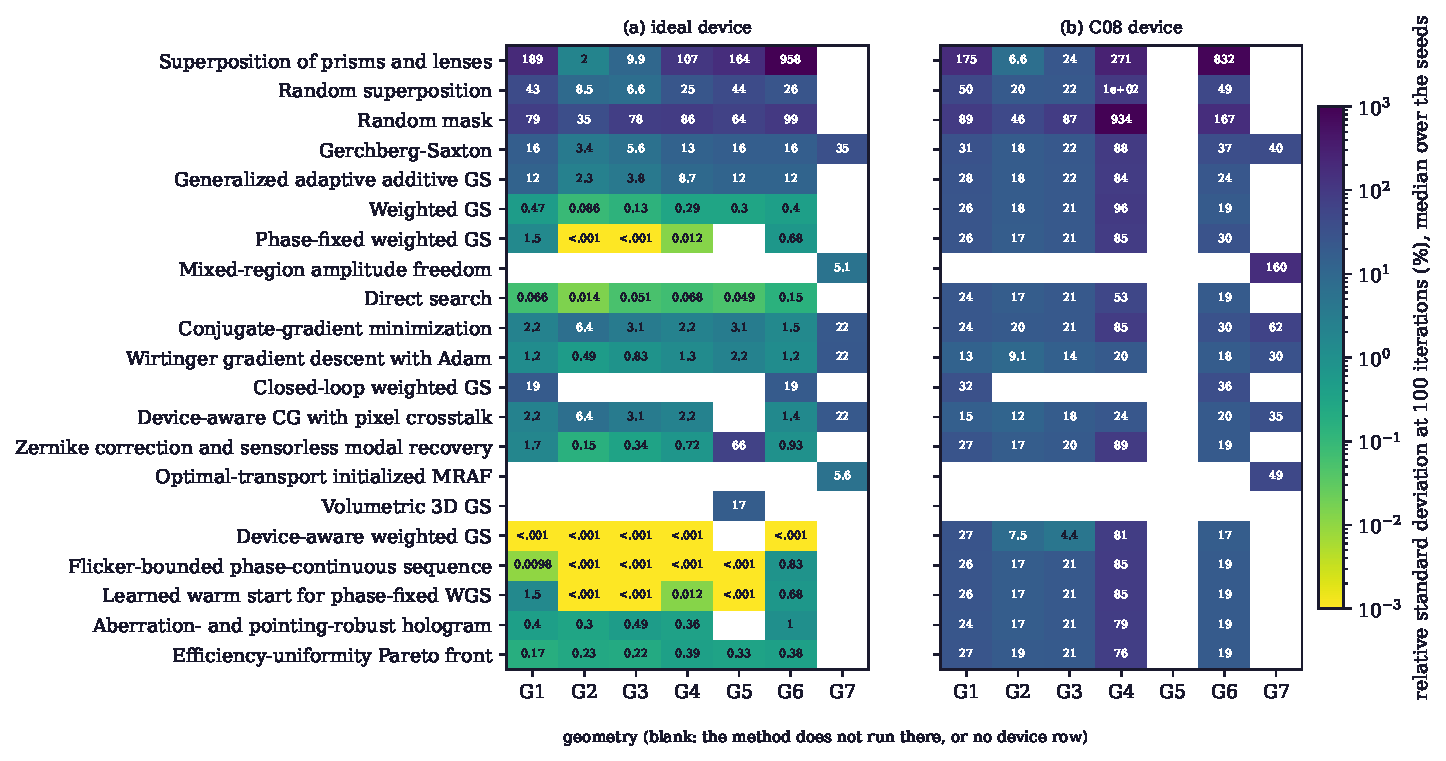
\includegraphics[width=\textwidth]{fig-bench.pdf}
\caption{Benchmark: median relative standard deviation at 100 iterations with the default parameters, every method on every geometry, on the ideal device (a) and on the C08 device (b). Blank: the method does not accept the geometry or refuses it, or the geometry has no device row.}
\label{fig:bench}
\end{figure}

Figure~\ref{fig:geometry} reads the same cells by geometry. On the ideal device the medians of the methods spread over several orders of magnitude within one geometry, from the analytic baselines to the optimization methods, and the proposed methods sit at the low end together with the phase-fixed and direct-search methods; on the C08 device the medians are compressed into a band of about one decade, with the geometry that has no device rows blank and no method below a few percent, a floor set by the quantizer and the flicker, which no method models completely. The figure does not show the efficiency of each point, which Table~\ref{tab:benchmethods} gives, and it does not show the seed-to-seed interval, which is in the results file.

\begin{figure}[t]
\centering
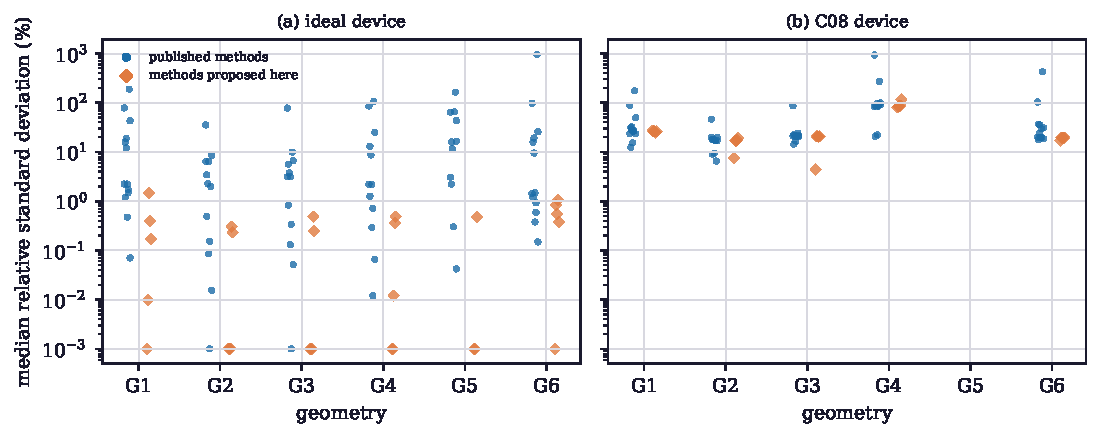
\includegraphics[width=\textwidth]{fig-geometry.pdf}
\caption{Median relative standard deviation at 100 iterations of every method on each point-trap geometry of the benchmark, on the ideal device (a) and on the C08 device (b); blue circles are the published methods and orange diamonds the methods proposed here. The vertical axis is logarithmic and the horizontal position within a geometry only separates the two groups.}
\label{fig:geometry}
\end{figure}

\subsection{The learned models}\label{sec:learned}

Two networks were trained offline with PyTorch, exported to ONNX with a list of operators the browser runtime supports, and evaluated on held-out sets written before the final training with other seeds. A model is released only if it meets its criterion; otherwise the baseline answers. The first network (Section~\ref{sec:m17}) maps three plane amplitudes at $-8$, $0$ and $+8$ SLM-limited Rayleigh ranges to one phase for the $128\times128$ SLM, in the setting of DeepCGH~\cite{eybposh}. It is trained without labels through the differentiable Fourier model with the loss $1-\mathrm{AC}$ of Eq.~\eqref{eq:m17} for \cghSteps{} steps. The exported graph is \cghBytes{} MB. The baseline is the volumetric three-dimensional GS on the same traps with a wall-clock budget of \cghBudgetS{} s, the median time of the volumetric GS at 30 iterations. On \cghN{} held-out volumes the network answers in about \cghNetMs{} ms with a median accuracy ratio of \cghMed{} (quartiles \cghQOne{} and \cghQThree{}), above the baseline on \cghShareAbove{} percent of the volumes; the median accuracy is \cghAcHybrid{} against \cghAcMnine{}. By kind the ratio is \cghLatticeRatio{} (lattices), \cghRandomRatio{} (random), \cghMixedRatio{} (mixed), \cghRingRatio{} (rings), \cghGfiveRatio{} (the $5\times5\times3$ benchmark lattice) and \cghPlaneRatio{} (the three-plane layout). The graph agrees with its training framework on the reconstructed plane intensities to $\cghParity$ relative to the maximum. The accuracy measure scores full plane images, ghosts and blur included, which is what the network optimises; the volumetric GS optimises trap uniformity, so the ratio is a statement about this measure. The two-dimensional counterpart, a single-plane network followed by GS refinement, ties: on \cghTwoDN{} held-out targets the ratio at equal wall-clock is \cghTwoDMed{}, below the criterion, and that model is not released.

The second model is a permutation-equivariant set network that predicts initial trap phases for phase-fixed weighted GS (Section~\ref{sec:b3}). On \wsN{} held-out geometries it needs a median of \wsModelIt{} iterations to reach one percent against \wsRandomIt{} from a random start (a factor of \wsRatio{}, below the factor of two set as the criterion), but only with the early phase freeze (after \wsNfixModel{} iterations, against \wsNfixRandom{} for the random arm). A control with no network, a random start and the same early freeze, needs a median of \wsControlIt{} iterations on the control subset, and \wsControlNever{} percent of its geometries never reach one percent (\wsModelNever{} percent with the network); the final efficiency differs by \wsEffDiff{} percent between the arms. The gain comes from the freeze, not from the network, so the proposal is refuted and the model is not released (Figure~\ref{fig:learned}). The panel (b) of the figure shows the three arms, and does not show the share that never converges, which the text gives.

\begin{figure}[t]
\centering
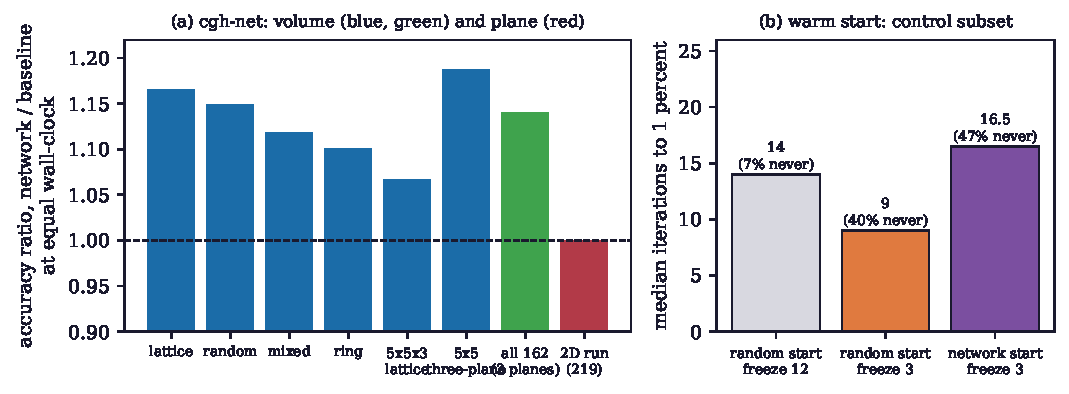
\includegraphics[width=\textwidth]{fig-learned.pdf}
\caption{(a) The cgh-net accuracy ratio over its baseline at equal wall-clock, by target kind on the held-out volumes (G5: the $5\times5\times3$ lattice; 3-plane: the $5\times5$ three-plane layout), for the volume network (blue, green) and the two-dimensional single-plane network (red); the dashed line is the baseline. (b) The warm-start control: median iterations to 1 percent for a random start with the original and the early freeze and for the network start with the early freeze.}
\label{fig:learned}
\end{figure}

\subsection{Ablations, sensitivities and the Pareto fronts}\label{sec:results-ablation}

Three sensitivities were measured, one per method whose result depends on a parameter that the source sets differently. The first is the freeze index of the phase-fixed weighted GS on a crowded array (Table~\ref{tab:nfix}, Figure~\ref{fig:nfix}): the minimum spread reached in 150 iterations falls as the index rises, from a stall at the source value to a value below the target at the larger values, and with $N=60$ the phase-fixed form reaches 0.5 percent in fewer iterations than weighted GS on both seeds (\acc{pfwgs}). The reading is that the phase frozen after a few iterations belongs to an unconverged hologram on this grid, and the weight update then cannot repair it; the table shows that the dependence is not monotone at the largest value, so the optimum depends on the grid and the budget. The second is the scale convention of the adaptive form (Section~\ref{sec:m05}): with the printed bracket the uniformity falls below GS, and with the scale convention it rises above it on every seed. The third is the target level of the aberration-robust hologram (Section~\ref{sec:b4}), which trades efficiency for robustness: a higher level gives a smaller improvement factor. Among the components of the device-aware weighted GS (Section~\ref{sec:b1}) the safeguard that returns the best admissible iterate is what makes the method never worse than its start, and the quantizer treated straight-through is the component that costs more than it gives on case C08. The fourth component, the weight update, was ablated (Table~\ref{tab:b1-weights}, measured for the companion manuscript): with every weight kept at one the relative standard deviation is lower on the acceptance task and on the square lattice of the C08 device, higher on the ring, and the same on the random and quasi-periodic sets, so that the weight update is not shown to be needed and the method is reported with the weights it is defined with.

\begin{table}[t]\centering\footnotesize
\caption{Phase-fixed weighted GS on the crowded $50\times30$ array: the minimum relative standard deviation reached in 150 iterations against the freeze index $N$ (one seed, Fourier form), measured by \texttt{acceptance.py}. The source value does not transfer to this grid.}\label{tab:nfix}
\begin{tabular}{@{}r r@{}}\toprule $N$ & minimum $\sigma$ (percent)\\\midrule
12 & 3.575\\
20 & 2.133\\
30 & 0.855\\
40 & 0.080\\
60 & 0.143\\
\bottomrule\end{tabular}\end{table}


\begin{table}[t]\centering\footnotesize
\caption{Ablation of the weight update of the device-aware weighted GS (B1), the method run with its weight update and with every weight kept at one. First block: the $10\times10$ acceptance task, median [min, max] of the relative standard deviation $\sigma$ (\%) over the seeds. Second block: the four benchmark geometries on the C08 device at 10 outer iterations, median over three seeds of $\sigma$ and of the efficiency $e$.}\label{tab:b1-weights}
\begin{tabular}{@{}l r r r r@{}}\toprule Task & $\sigma$ with weights & $\sigma$ no weights & $e$ with & $e$ no weights\\\midrule
acceptance task, crosstalk device (5 seeds) & 0.205 [0.157, 0.298] & 0.0297 [0.0163, 0.0319] & & \\
acceptance task, 4-bit device (3 seeds) & 0.724 [0.597, 1.16] & 0.242 [0.202, 0.248] & & \\
G1 10 x 10 square (C08 device, 3 seeds) & 29 & 14 & 0.598 & 0.563\\
G2 ring of 36 (C08 device, 3 seeds) & 7.8 & 8.9 & 0.453 & 0.464\\
G3 100 random (C08 device, 3 seeds) & 4.4 & 4.3 & 0.401 & 0.408\\
G4 quasi-periodic 119 (C08 device, 3 seeds) & 65 & 65 & 0.493 & 0.493\\
\bottomrule\end{tabular}\end{table}


\begin{figure}[t]
\centering
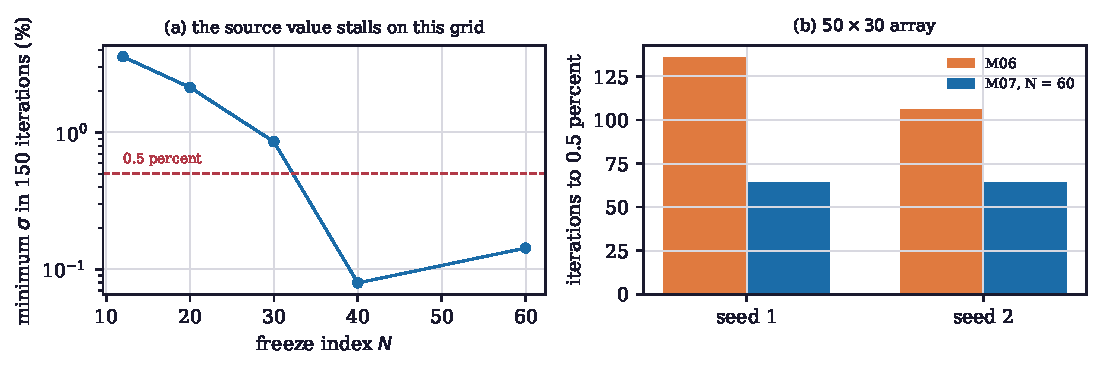
\includegraphics[width=\textwidth]{fig-nfix.pdf}
\caption{Phase-fixed weighted GS on the crowded $50\times30$ array: (a) the minimum relative standard deviation in 150 iterations against the freeze index $N$, with the target of 0.5 percent dashed; (b) iterations to reach 0.5 percent for weighted GS and for the phase-fixed form ($N=60$) on the two seeds of the acceptance test.}
\label{fig:nfix}
\end{figure}

The fronts of the efficiency--uniformity method are the last measured outcome (Table~\ref{tab:pareto}, Figure~\ref{fig:pareto}). On the ideal device the stored fronts are short: they hold between one and seven non-dominated points, and from the first to the last stored point the efficiency changes by at most a few hundredths while the uniformity changes by a few hundredths at most on the lattice geometries and not at all where a single point is stored. The weighted-GS corner is already near the optimum of the trade-off, so the front is nearly flat in this region, which is the risk that the design had named. The figure shows the front against the single points of the published methods at 100 iterations, so that a reader sees which points the front dominates; it does not show the hypervolume, which the table of the benchmark counts per geometry in Section~\ref{sec:results-bench}.

\begin{table}[t]\centering\footnotesize
\caption{Stored Pareto fronts of the benchmark (the converged run of the first seed, non-dominated points only): the number of stored points, and the efficiency $e$ and uniformity $u$ of the first and of the last stored point ordered by the trade-off parameter, per geometry with a front, on the ideal device.}\label{tab:pareto}
\begin{tabular}{@{}l r r r r r@{}}\toprule Geometry & Points & $e$ first & $u$ first & $e$ last & $u$ last\\\midrule
G1 & 7 & 0.822 & 1.000 & 0.838 & 0.947\\
G2 & 2 & 0.693 & 1.000 & 0.699 & 0.998\\
G3 & 3 & 0.692 & 1.000 & 0.708 & 0.997\\
G4 & 3 & 0.751 & 1.000 & 0.766 & 0.991\\
G5 & 3 & 0.859 & 1.000 & 0.893 & 0.995\\
G6 & 1 & 0.791 & 1.000 & 0.791 & 1.000\\
\bottomrule\end{tabular}\end{table}


\begin{figure}[t]
\centering
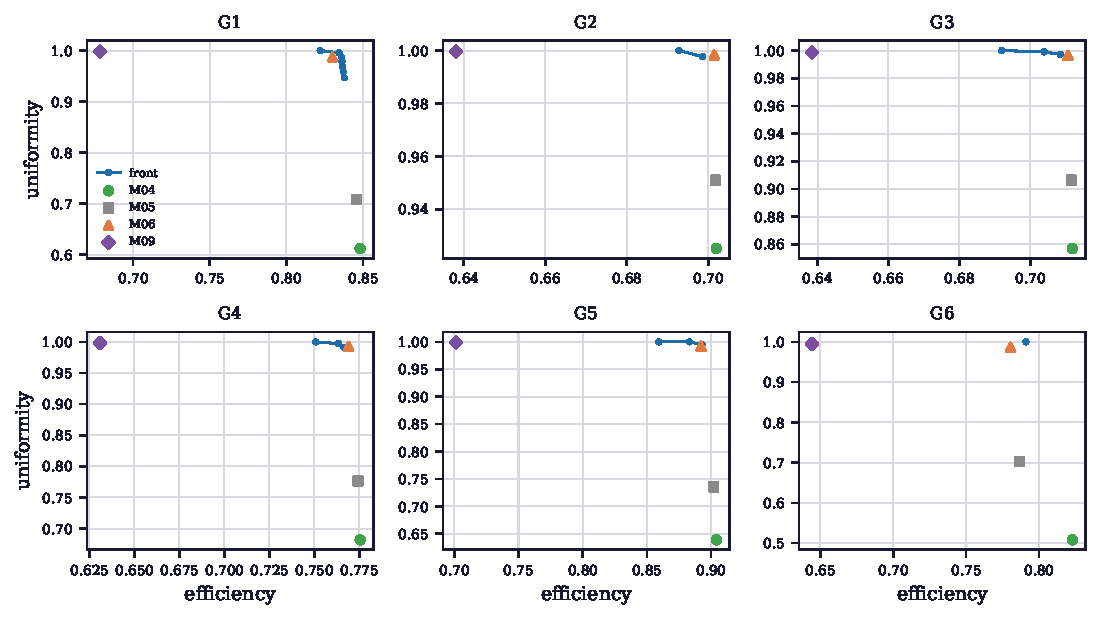
\includegraphics[width=\textwidth]{fig-pareto.pdf}
\caption{Stored efficiency--uniformity fronts of the benchmark on the ideal device, one panel per geometry with a front, against the median efficiency and uniformity at 100 iterations of the published methods GS, the adaptive form, weighted GS and direct search on the same geometry.}
\label{fig:pareto}
\end{figure}

\subsection{Summary of the proposed methods}\label{sec:results-proposed}

Of the five proposed methods, three meet their acceptance criteria on their acceptance tasks, each within a scope that the benchmark or the scope measurements narrow (a device-aware weighted GS update, a flicker-bounded phase-continuous sequence and an efficiency--uniformity front), one meets a narrowed criterion (an aberration-robust hologram, whose pointing-error clause is not obtained in the acceptance configuration and is reached only with a displacement prior optimized alone at five times the budget) and one is refuted by measurement (a learned warm start for phase-fixed weighted GS). The device-aware method is measured on the device of C08 over \benchOnePass{} of \benchOneN{} geometries (\benchOnePassList), where it meets both thresholds, and the front's stored result reaches the hypervolume of the published points on \benchFivePass{} of the \benchFiveN{} geometries at 100 iterations and on \benchFivePassThirty{} at 30. The details of the device-aware weighted GS and of the flicker-bounded sequence, with the factor on each geometry and the long moves of the sequence, are in the companion manuscript~\cite{companion}; the outcome of each of the five is the same one that its method section states, and none is reported as better than it measured. The summary does not rank the five against each other, because their criteria are different quantities on different tasks, and it does not extend any of them beyond the tasks and the device on which it was measured. The measured acceptance of the aberration-robust hologram and the Pareto front is in Table~\ref{tab:acceptance} (\acc{paretofront}).
